\PassOptionsToPackage{unicode=true}{hyperref} % options for packages loaded elsewhere
\PassOptionsToPackage{hyphens}{url}
%
\documentclass[]{article}
\usepackage{lmodern}
\usepackage{amssymb,amsmath}
\usepackage{ifxetex,ifluatex}
\usepackage{fixltx2e} % provides \textsubscript
\ifnum 0\ifxetex 1\fi\ifluatex 1\fi=0 % if pdftex
  \usepackage[T1]{fontenc}
  \usepackage[utf8]{inputenc}
  \usepackage{textcomp} % provides euro and other symbols
\else % if luatex or xelatex
  \usepackage{unicode-math}
  \defaultfontfeatures{Ligatures=TeX,Scale=MatchLowercase}
\fi
% use upquote if available, for straight quotes in verbatim environments
\IfFileExists{upquote.sty}{\usepackage{upquote}}{}
% use microtype if available
\IfFileExists{microtype.sty}{%
\usepackage[]{microtype}
\UseMicrotypeSet[protrusion]{basicmath} % disable protrusion for tt fonts
}{}
\IfFileExists{parskip.sty}{%
\usepackage{parskip}
}{% else
\setlength{\parindent}{0pt}
\setlength{\parskip}{6pt plus 2pt minus 1pt}
}
\usepackage{hyperref}
\hypersetup{
            pdftitle={Untitled},
            pdfauthor={Some authors},
            pdfborder={0 0 0},
            breaklinks=true}
\urlstyle{same}  % don't use monospace font for urls
\usepackage[margin=1in]{geometry}
\usepackage{longtable,booktabs}
% Fix footnotes in tables (requires footnote package)
\IfFileExists{footnote.sty}{\usepackage{footnote}\makesavenoteenv{longtable}}{}
\usepackage{graphicx,grffile}
\makeatletter
\def\maxwidth{\ifdim\Gin@nat@width>\linewidth\linewidth\else\Gin@nat@width\fi}
\def\maxheight{\ifdim\Gin@nat@height>\textheight\textheight\else\Gin@nat@height\fi}
\makeatother
% Scale images if necessary, so that they will not overflow the page
% margins by default, and it is still possible to overwrite the defaults
% using explicit options in \includegraphics[width, height, ...]{}
\setkeys{Gin}{width=\maxwidth,height=\maxheight,keepaspectratio}
\setlength{\emergencystretch}{3em}  % prevent overfull lines
\providecommand{\tightlist}{%
  \setlength{\itemsep}{0pt}\setlength{\parskip}{0pt}}
\setcounter{secnumdepth}{0}
% Redefines (sub)paragraphs to behave more like sections
\ifx\paragraph\undefined\else
\let\oldparagraph\paragraph
\renewcommand{\paragraph}[1]{\oldparagraph{#1}\mbox{}}
\fi
\ifx\subparagraph\undefined\else
\let\oldsubparagraph\subparagraph
\renewcommand{\subparagraph}[1]{\oldsubparagraph{#1}\mbox{}}
\fi

% set default figure placement to htbp
\makeatletter
\def\fps@figure{htbp}
\makeatother

\usepackage{setspace}\doublespacing

\title{Untitled}
\author{Some authors}
\date{}

\begin{document}
\maketitle

\hypertarget{abstract}{%
\subsection{Abstract}\label{abstract}}

\hypertarget{introduction}{%
\subsection{Introduction}\label{introduction}}

Background info/research on breast cancer patients:

Breast cancer occurs due to abnormal cell growths in breast tissue.
Although it is most often found in females, 1 out of every 100 diagnosed
patients in the US is a male. Other breast cancer risk factors include,
increase in age, family history or personal history of breast cancer,
radiation exposure, obesity, alcohol use, among many more. Research
suggests that postmenopausal hormone therapy is a risk factor due the
combination of estrogen and progesterone used to treat signs and
symptoms of menopause.

Additionally, the patient's breast cancer stage is important to consider
when determining the severity of the cancer and how to treat it. The
American Joint Committee on Cancer (AJCC) TNM system is the most common,
and contains clinical and pathologic systems. The pathologic stage is
determined by examining the tissue removed during surgery, while the
clinical stage is based on results of a physical exam, biopsy, and
imaging tests. Nevertheless, both systems are composed of the size of
the tumor, the spread to nearby lymph nodes and/or to distant sites,
their estrogen and/or progesterone receptor status, the grade of the
cancer, and if the cancer makes too much of HER2 protein.

Although, most recently, breast cancer survival rates have increase and
number of deaths decreased, it would be important to explore the risk
factors of breast cancer. For this project, we will investigate the odds
of breast cancer survival given most of the risk factors previously
mentioned.

\hypertarget{methods}{%
\subsection{Methods}\label{methods}}

\hypertarget{data-source}{%
\paragraph{Data source}\label{data-source}}

We obtained a deidentified set containing data on 4024 breast cancer
patients. this dataset contains both demographic information, such as
patient age, race, and marital status; clinical information such as
tumor stage, tumor size, hormone therapies (progesterone and estrogen),
regional node positive, and regional node examined; and outcome
information: the number of months the patient had survived prior to
study conclusion, and their alive/dead status at the end of the study.

\hypertarget{data-cleaning}{%
\paragraph{Data cleaning}\label{data-cleaning}}

We combined the regional node positive and regional node examined
variables into a ``regional node proportion positive'' variable. This
variable, but neither the node positive nor node examined variables were
in the model. Further, we decided to discard the T stage and N stage
variables, as they captured information already contained in the AJCC
6th stage variable. We also excluded the grade variable, as it captured
the same clinical information as the differentiate variable. Due to the
skewness in the distribution of the tumor size, we applied a square root
transformation to that variable (\textbf{Supplemental Figure 1}). We
also added a \texttt{main\_stage} variable, which groups all the stages
in \texttt{6th\_stage} so that ``IIIA'' and ``IIIC'' are under factor
level ``III'' for example, and added a \texttt{white} variable that
tells us if the patient is ``White'' or not, essentially grouping
``Black'' and ``Other'' together. Both variables were created in case
the reduction of factor levels makes the fit better.

\hypertarget{model-construction}{%
\paragraph{Model construction}\label{model-construction}}

We decided to use logistic regression model to estimate the risk of
patient death within the followup window. Formally, we assumed that an
for an individual, with probability \emph{p} to die after receiving a
breast cancer diagnosis, the log-odds of \emph{p} was linear, i.e.

\(logit(p_i) = \mathbf{X}\beta+ \epsilon_i\)

Where \textbf{\emph{X}} is the n x p design matrix, and \(\beta\) is a
vector in \(\mathbb{R}^p\).

In addition to the covariates we included the interaction between
\texttt{estrogen\_status} and \texttt{progesterone\_status} given that
we found in our background research that having both ``positive''
increase the chances of breast cancer.

\hypertarget{model-selection}{%
\paragraph{Model selection}\label{model-selection}}

We considered all We used a criterion-based method, utilizing Akaike
Information Criterion (AIC) to assess the performance of our models.

\hypertarget{model-validation}{%
\paragraph{Model validation}\label{model-validation}}

We performed 10 cross-validation to assess the performance of our model.
Each observation in a dataset will be in 1 of 10 folds such that it gets
used as training data 9 times, and as test data once. The predictions
are then saved such that each row has an out-of-sample prediction that
can be compared to the real value.

\hypertarget{table-1.}{%
\paragraph{Table 1.}\label{table-1.}}

This table shows the confusion matrix made from our 10 fold
cross-validation, such that the predicted values are out-of-sample
predictors. We can see that the model is very good at correctly
predicting that somebody survived, and rarely predicts the individual
died when it didn't. However, the model makes a lot of errors when
trying to predict if the individual survived: more than 90\% of the
total error happens when the model predicts the individual died, and it
actually survived. This reflects the fact that the model prefers to
predict 0 as a result of the \texttt{status} variable being 0 inflated.

\begin{longtable}[]{@{}lrr@{}}
\toprule
& Predicted Died & Predicted Survived\tabularnewline
\midrule
\endhead
Actually Died & 3357 & 51\tabularnewline
Actually Survived & 533 & 83\tabularnewline
\bottomrule
\end{longtable}

\hypertarget{software}{%
\paragraph{Software}\label{software}}

The aforementioned analyses were carried out using R 4.3.1 and RStudio
Version 2023.06.2+561.

\hypertarget{results}{%
\subsection{Results}\label{results}}

\hypertarget{model-construction-and-selection}{%
\paragraph{Model construction and
selection}\label{model-construction-and-selection}}

We used a logistic model coupled with criterion-based stepwise
regression to determine which variables were useful in predicting the
risk of death in breast cancer patients. The variables that were
identified as important were age, race, marital status, AJCC 6th stage,
differentiate, estrogen status, progesterone status, tumor size, and
regional node positive proportion. The variables that were not
identified as important by the model were whether the tumor was Stage A
and the interaction between estrogen and progresterone status. For a
list of model coefficients see \textbf{Supplemental Table 1}.

\hypertarget{diagnostics}{%
\paragraph{Diagnostics}\label{diagnostics}}

ROC, Brier score

ROC for full model on in-sample data:

\includegraphics[width=0.9\linewidth]{written_report_files/figure-latex/roc curve-1}

\begin{verbatim}
## Area under the curve: 0.7542
\end{verbatim}

Separation plots

\hypertarget{model-performance-by-race}{%
\paragraph{Model performance by race}\label{model-performance-by-race}}

Make a table with ROC AUC and Brier scores by race. Discuss

\begin{longtable}[]{@{}lrr@{}}
\toprule
race & roc\_auc & brier\_score\tabularnewline
\midrule
\endhead
White & 0.760 & 0.109\tabularnewline
Black & 0.704 & 0.171\tabularnewline
Other & 0.650 & 0.088\tabularnewline
\bottomrule
\end{longtable}

\hypertarget{discussion}{%
\subsection{Discussion}\label{discussion}}

\hypertarget{author-contributions}{%
\subsection{Author Contributions}\label{author-contributions}}

\hypertarget{references}{%
\subsection{References}\label{references}}

\newpage

\hypertarget{appendices}{%
\subsection{Appendices}\label{appendices}}

\begin{enumerate}
\def\labelenumi{\alph{enumi}.}
\tightlist
\item
  tumor size transformation
\end{enumerate}

\begin{verbatim}
## `stat_bin()` using `bins = 30`. Pick better value with `binwidth`.
## `stat_bin()` using `bins = 30`. Pick better value with `binwidth`.
\end{verbatim}

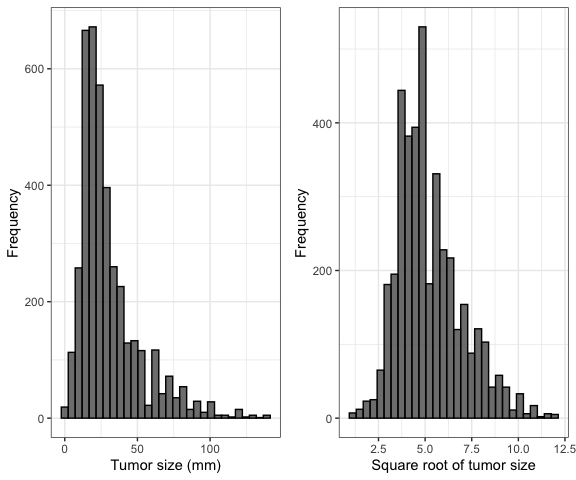
\includegraphics[width=0.9\linewidth]{written_report_files/figure-latex/tumor size transformation hist-1}

\textbf{Figure S1.} Transformation of tumor size variable. (A) Before
transformation. (B) After square root transformation.

\begin{enumerate}
\def\labelenumi{\alph{enumi}.}
\setcounter{enumi}{1}
\tightlist
\item
  model coefficients
\end{enumerate}

\hypertarget{table-s1.-model-coefficients}{%
\paragraph{Table S1. Model
Coefficients}\label{table-s1.-model-coefficients}}

\begin{longtable}[]{@{}lrrrr@{}}
\toprule
term & estimate & std.error & statistic & p.value\tabularnewline
\midrule
\endhead
(Intercept) & -4.197 & 0.369 & -11.382 & 0.000\tabularnewline
age & 0.023 & 0.006 & 4.180 & 0.000\tabularnewline
raceBlack & 0.506 & 0.162 & 3.129 & 0.002\tabularnewline
raceOther & -0.431 & 0.202 & -2.132 & 0.033\tabularnewline
marital\_statusDivorced & 0.222 & 0.141 & 1.575 & 0.115\tabularnewline
marital\_statusSingle & 0.153 & 0.134 & 1.146 & 0.252\tabularnewline
marital\_statusWidowed & 0.225 & 0.192 & 1.171 & 0.242\tabularnewline
marital\_statusSeparated & 0.847 & 0.366 & 2.316 & 0.021\tabularnewline
x6th\_stageIIIA & 0.563 & 0.163 & 3.460 & 0.001\tabularnewline
x6th\_stageIIIC & 1.064 & 0.193 & 5.505 & 0.000\tabularnewline
x6th\_stageIIB & 0.413 & 0.154 & 2.676 & 0.007\tabularnewline
x6th\_stageIIIB & 1.141 & 0.322 & 3.546 & 0.000\tabularnewline
differentiateModerately differentiated & -0.389 & 0.104 & -3.726 &
0.000\tabularnewline
differentiateWell differentiated & -0.919 & 0.192 & -4.776 &
0.000\tabularnewline
differentiateUndifferentiated & 0.961 & 0.529 & 1.816 &
0.069\tabularnewline
estrogen\_statusNegative & 0.738 & 0.177 & 4.169 & 0.000\tabularnewline
progesterone\_statusNegative & 0.571 & 0.127 & 4.485 &
0.000\tabularnewline
root\_tumor\_size & 0.048 & 0.031 & 1.523 & 0.128\tabularnewline
regional\_prop & 1.237 & 0.185 & 6.686 & 0.000\tabularnewline
\bottomrule
\end{longtable}

\begin{enumerate}
\def\labelenumi{\alph{enumi}.}
\setcounter{enumi}{1}
\tightlist
\item
  ROC by race +/- sep plots?
\end{enumerate}

\end{document}
